\documentclass[12pt]{guia}
\grade{3$^\circ$ de Secundaria}
\cycle{2022-2023}
\subject{Química 3}
\guide{2}
\title{Geometría molecular}
\aprendizajes{
    \begin{itemize}[leftmargin=*,label=\small\color{colorrds}\faIcon{user-graduate}]
        \item Explica y predice propiedades físicas de los materiales con base con base en modelos
        submicroscópicos sobre la estructura de átomos, moléculas o iones, y sus interacciones
        electrostáticas.
    \end{itemize} 
}
\requisitos{
    \begin{itemize}
        \item Requisito 1
        \item Requisito 2
    \end{itemize}
}
\author{J. C. Melchor Pinto}

\begin{document}
\pagestyle{headandfoot}
\addpoints
\INFO
%\printanswers
\begin{opening}[Geometría molecular]
    {
        \begin{minipage}{.2\textwidth}
            \begin{figure}[H]
                \centering
                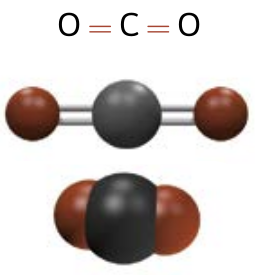
\includegraphics[width=.9\linewidth]{../images/fig2.38.png}
                \caption{Diferentes representaciones de la geometría lineal de la molécula de dióxido de carbono (CO$_2$) .}
                \label{fig:2.38}
            \end{figure}
        \end{minipage}\hfill
        \begin{minipage}{.55\textwidth}
            Los materiales que nos rodean están hechos de diferentes sustancias, y sus propiedades dependen de su composición y de la estructura de las partículas que los
            componen. Como hemos visto, las moléculas que conforman las sustancias están
            compuestas por distintos tipos de átomos enlazados de diversas maneras, lo cual
            determina si el material que forman será o no soluble en agua, si a temperatura
            ambiente existirá como líquido o sólido o si lo atraerá o no un cuerpo cargado.
            El tipo de átomos que se combinan para formar una molécula y la manera en la
            que se enlazan determina la ``geometría'' de la partícula, es decir, la forma que adquiere; por ejemplo, las moléculas de dióxido de carbono (CO$_2$) están compuestas por
            un átomo de carbono unido mediante enlaces dobles a dos átomos de oxígeno organizados en una línea. Se dice entonces que la molécula tiene \textbf{geometría lineal} (figura \ref{fig:2.38}).
            No todas las moléculas compuestas por tres átomos son lineales. Las moléculas
            de agua H$_2$O, por ejemplo, poseen una \textbf{geometría plana angular} debido a repulsiones
            entre los electrones de valencia en el átomo de oxígeno central y en los átomos de
            hidrógeno que lo rodean (figura \ref{fig:2.39}).
        \end{minipage}\hfill
        \begin{minipage}{.2\textwidth}
            \begin{figure}[H]
                \centering
                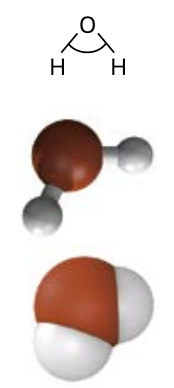
\includegraphics[width=.9\linewidth]{../images/fig2.39.png}
                \caption{Distintas representaciones de la geometría plana de la molécula
                    de H$_2$O.}
                \label{fig:2.39}
            \end{figure}
        \end{minipage}
    }
\end{opening}
\begin{questions}
    \include*{../questions/question006}
    \begin{minipage}{.4\textwidth}
        \begin{figure}[H]
            \centering
            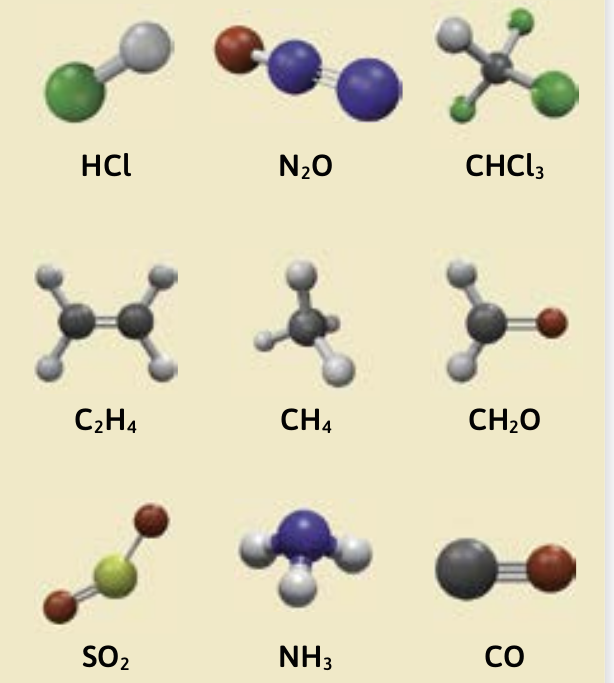
\includegraphics[width=.85\linewidth]{../images/geometrias_moleculas}
            \caption{Geometría de algunas moléculas.}
            \label{fig:geometrias_moleculas}
        \end{figure}
    \end{minipage}\hfill
    \begin{minipage}{.55\textwidth}
        \include*{../questions/question004}
    \end{minipage}
    \include*{../questions/question005}
\end{questions}

%\vfill
%\puntuacion

\end{document}